\documentclass[10pt,twocolumn,letterpaper]{article}

\usepackage{cvpr}
\usepackage{times}
\usepackage{epsfig}
\usepackage{graphicx}
\usepackage[font=small,labelfont=bf]{caption}
\usepackage{amsmath}
\usepackage{amssymb}
\usepackage{float}

% Include other packages here, before hyperref.

% If you comment hyperref and then uncomment it, you should delete
% egpaper.aux before re-running latex.  (Or just hit 'q' on the first latex
% run, let it finish, and you should be clear).
\usepackage[breaklinks=true,bookmarks=false]{hyperref}

\cvprfinalcopy % *** Uncomment this line for the final submission

\def\cvprPaperID{****} % *** Enter the CVPR Paper ID here
\def\httilde{\mbox{\tt\raisebox{-.5ex}{\symbol{126}}}}

% Pages are numbered in submission mode, and unnumbered in camera-ready
%\ifcvprfinal\pagestyle{empty}\fi
\setcounter{page}{1}
\begin{document}

%%%%%%%%% TITLE
\title{What's this books genre?}

\author{Hakan AKYUREK\\
Hacettepe University\\
21426553\\
{\tt\small akyurekhakanarbeit@gmail.com}
% For a paper whose authors are all at the same institution,
% omit the following lines up until the closing ``}''.
% Additional authors and addresses can be added with ``\and'',
% just like the second author.
% To save space, use either the email address or home page, not both
\and
Sefa YURTSEVEN\\
Hacettepe University\\
21427559\\
{\tt\small yurtsevensefa14@gmail.com}
}

\maketitle
%\thispagestyle{empty}

%%%%%%%%% ABSTRACT
\begin{abstract}
In this paper we discuss various approaches for predicting a book's genre from it's summary, that is predicting multiple genres for each book only looking to their summaries. We implemented an ANN model to achieve our goal. We experimented with CMU Book Summaries dataset with 16000 book summaries along with their respective authors and multiple genres. We worked on multi-label text classification problem, tried different input representations like bag of words and word2vec. In multi-label classification basically each data corresponds to multiple somehow related classes, however, it should not be confused with multi-class classification, which is a different topic. We have also worked on a side model, namely label powerset, to better evaluate our ANN model and compare them. Evaluation of our models are done with numerous metrics like hamming loss, accuracy or our own metrics.
\end{abstract}

%%%%%%%%% BODY TEXT
\section{Introduction}

Finding book genres from their summaries is a different topic that challenges us with some of the  not so common NLP and Machine Learning problems. The problem in question is quite challenging and as much as interesting as it requires working with a highly imbalanced multi-labelled dataset, which requires different textual input representations, evaluation metrics to have a better understanding of the models, and multi-label algorithms which we couldn't find a chance to work with before.

Book genre prediction is a rather unique problem, while being a variation of a multi-labelled text classification problem. It is important in cases such as: library documentation or book store database construction. Recently, many researches worked on the problem of multi-labelled text classification or multi-label classification in general. So, some algorithms have been devised for multi-label classification. Common approaches include 'Label Power Set', 'Binary Relevance', 'Artificial Neural Networks' and so on.

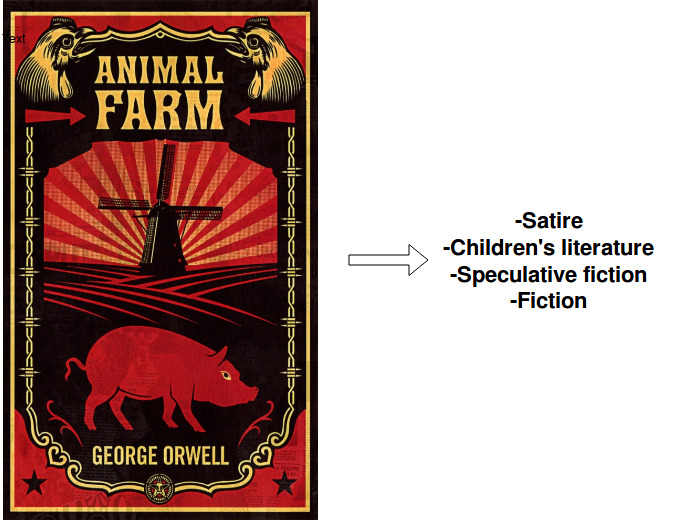
\includegraphics[width=0.8\linewidth]{Book}

Representation of textual data was also one of our research topics. We used vectorised text documents, either with BoW or Word2Vec, to feed our ANN and other models. The vectorised documents go through some preprocessing before being fed to a model. We have also analysed how our models respond to different input representations.

In this study we came up with our own approach to multi-label classification. We have also came up with our own metric to evaluate our models and used other metrics such as: accuracy, hamming loss, and zero-one loss.

Main contributions can be considered as such:
\begin{itemize}
\item[-] Classification of multi-label data and its evaluation.
\item[-] Analysis of numerous input representations, evaluation metrics, multi-label models.
\end{itemize}

We should note, however, we didn't try to solve the imbalance issue of our dataset. There are some re-sampling techniques are being researched by the researchers like Cocoa approach, but it was out of the scope of our project.\\

The rest of the paper is as follows. We briefly review the related studies in Sec. 2. In Sec. 3 we describe our approach in detail. Results of experiments are discussed in Sec. 4. Then, we discuss our conclusions in Sec. 5.

\section{Related Works}
According to imbalanced dataset problem, we have checked this paper\cite{Imb} and this paper\cite{Imb2}.

We also researched about multi-label text classification in literature. This paper\cite{movie} discusses predicting movie genres from their plot summaries using various methods and analyses their performance. Along with the Bag of words model we have also used word2vec model. The papers we checked can be found here\cite{DBLP:journals/corr/abs-1301-3781}. We have also checked doc2vec\cite{doc2vec} models, but we could not find a pre-trained model for that so we just skipped working with doc2vec.

We have used sk-multilearn\cite{2017arXiv170201460S} library, which is a amazing library providing numerous models for multi-label classification problems, to create our side model with Label powerset. 

We used artificial neural networks as our models, some of the examples can be found here\cite{annml1}, there\cite{annml3}. We have also found out using different loss functions from this issue in github\cite{annml2}.

Sklearn library\cite{scikit-learn}\cite{sklearn_api} also provides amazing metrics for us, researches to use. Hamming\cite{hammingloss} loss can be considered as our main metric in this project. The wikipedia entry\cite{hammingdistance} for hamming distance is also a site we checked.

There are some research done about how word2vec model and doc2vec model would benefit us. We found out using these models we can actually get compositional semantics of the documents. We checked out this\cite{comp1}, this\cite{comp2}.

\section{Our Approach}
In this study aim is to analyse various methods' and approaches' performance on classifying book genres using their summaries. Accordingly, the goal is to predict book genres as accurate as possible, again, using only their summaries. Obviously, one can see that a book cannot be classified to only one genre, so our problem is a multi-label text classification problem. 

We present 2 different approaches to input representation: Word2Vec and Bag of Words. The model selection approaches are as follows: Label Powerset, ANN. Furthermore, we also present different approaches to evaluation of these models: Accuracy, Hamming Loss, Threshold-Based Accuracy.

\subsection{Input Representation}
Since it is a text classification problem, multiple approaches to represent input is available. We assume that different input representations can actually change the performance of our models. The models we tried are limited to 'Word2Vec' and 'Bag of Words'. We wanted to use 'Doc2Vec' as well, but our corpus is not large enough to train a good model and we couldn't find any good pre-trained doc2vec model. So we used Google's pre-trained word2vec model\cite{word2vecmodel} to represent each word in our documents. We took the average of sums of each word embedding, giving a non-zero static vector for words that are not in models dictionary, to represent our every document.
\begin{equation}
\vec{W} = \vec{W_1} + \vec{W_2} + \vec{W_3} + \textellipsis + \vec{W_n}
\end{equation}	
\begin{equation}
\vec{D} = \frac{\vec{W}}{n}
\end{equation}
This way we are able to get compositional semantics of our documents. As it is discussed in "4. Experimental Results" it performs much better than bag of words model. If we had a doc2vec model we could extract these semantics much better, since with word2vec we are in a way not considering sequence of the words in a document. We are just looking to each words meaning. Then we feed those vectors to our models to train them. 

We also used bag of words to represent our data. But to use label powerset we need train and test data to have the same number of features, which we cannot achieve with bag of words. To solve this we have simply increase the number of features in the smaller one. This way we have the same number of features on both test and train data. We should note that, this problem does not occur in ANN. 

\subsection{Model Selection}
'Label powerset' is chosen as our side model in the project. Label powerset is a problem transformation approach, which transforms multi-label problem to a multi-class problem with 1 multi-class classifier trained on all unique label combinations found in the training data. We chose 'Random Forest Classifier' as the base classifier in this transformation method because, we believe that it will alleviate overfitting more than 'Multinomial Naive Bayes' or 'SVM' since it is a ensemble method, thus returning better results. 

As our main model, we chose 'Artificial Neural Networks'. While working on a multi-class problem we used softmax as activation and categorical crossentropy as loss function in our model before. But while working with a multi-label problem using these would be wrong and result in inaccurate outputs. Because, softmax transforms the output vector to a probability distribution. The problem is that with softmax each label's probability is dependent to others' probabilities. But with the sigmoid function we can achieve what we want, independent label probabilities, since it models the probability of a label as bernoulli distribution. To make this work with our 'keras' model we used binary crossentropy as loss function. Because we want to look at each output node independently.

\subsection{Evaluation Metrics}
Along with the pre-prepared metrics, we have also came up with our own approach while working with ANN. In a multi-label problem like this, expecting our model to predict every data with a 100\% would be cruel and somehow wrong, because if the model predicts 4 out of 5 labels correct it's also a highly correct prediction. So to check that we put a 'hit-rate' value of 0.65. If the total number of correctly predicted labels' percentage is higher than the hit-rate it can be considered as a correct prediction. By putting a hit-rate we basically say that predicting one of the labels correctly cannot be counted as a correct prediction. But, the question of how we can tell which labels can be counted as prediction. To solve that we put a 'threshold' value and only the labels in the output vector with higher probability than the threshold value are counted as a prediction. For example in a vector such as
\begin{verbatim}
 [0.01, 0.156, 0.063, 0.25, 0.23]
\end{verbatim} 
only the last 2 ones are considered a prediction when the threshold is 0.175. Giving a rather low threshold value would be incorrect since the algorithm will consider much more outputs as prediction and it would be inaccurate. Giving a rather high threshold value would be also incorrect, considering we have a total of 27 labels we do not expect our model to give output to certain labels even close to 0.5. To that respect, we gave 0.4 to our threshold value while evaluating our model.


\section{Experimental Results}

In this study we have tried many approaches, changed many hyper-parameters and evaluated them with different metrics. 

\subsection{Dataset Analysis}

We used a dataset created from wikipedia book database. The dataset contains 16000 books with some of their informations, which include publication date, author, summary, genres, and name. Most books have multiple, unequal number of genres while a huge number of books belong to only one genre. While exploring the dataset we came to a conclusion that we can't take every book in to account, since there are loads of books that belong to only one unique genre thus increasing our models error rate considerably. We took every genre with at least 100 books represented by them as it can be seen in Figure 1.

\begin{figure*}
\begin{center}
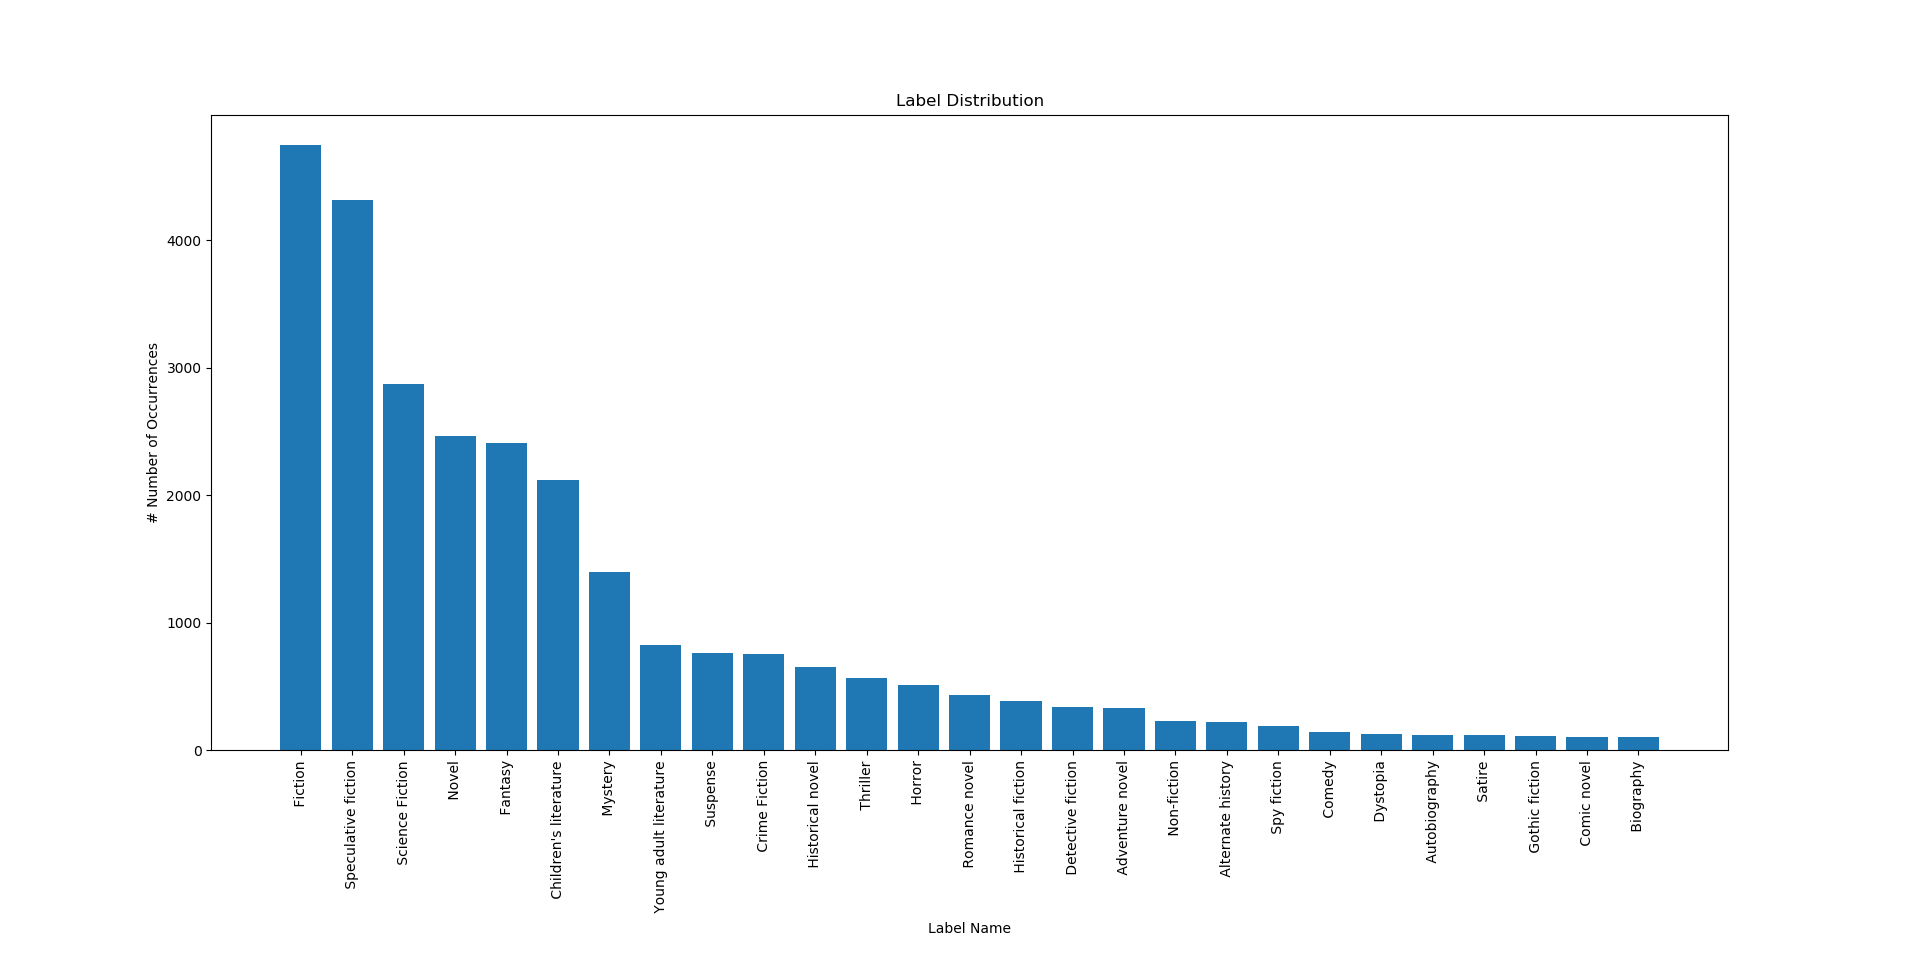
\includegraphics[width=1\linewidth]{BookDistributionPerGenre}
\end{center}
   \caption{Number of books represented by each label. Every genre represents at least 100 books.}
\label{fig:short}
\end{figure*}

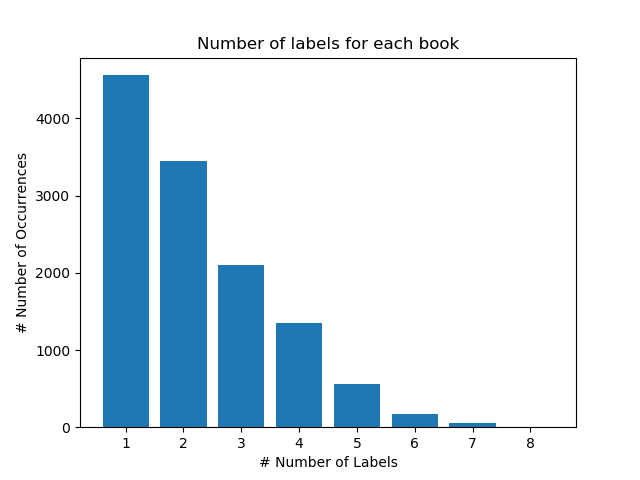
\includegraphics[width=1\linewidth]{LabelDistribution}
\captionof{figure}{4500 books with 1 label and 9 books with 8 labels.\\}

Further exploring our dataset, we found out a huge amount of books have only one genre. While at most in total 9 have 8 genres, around 4500 books have only 1 genre. Looking to Figure 2 and Figure 1 we can consider this a unique and rather interesting problem.

\subsection{Analysis of Input Representation}

Textual data can be represented in various ways: Bag of Words, Word2Vec, Doc2Vec. In this experiment we used Bag of Words and Word2Vec models to represent our data and analysed their effects on the performance of our models. Doc2Vec is not used as discussed in Section 3.1.\\

\begin{table}[H]
\begin{center}
\begin{tabular}{|c|c|c|}
\hline
& BoW & Word2Vec \\
\hline
Threshold-Based Accuracy & 20\% & 78\% \\
Hamming Loss & 0.043 & 0.036 \\
\hline
\end{tabular}
\end{center}
\caption{Different Input Representations on Artificial Neural Network}
\end{table}

Usage of Bag of Words really decreases the accuracy of our ANN model. It seems extracting information out of documents works far worse than getting the data structure of the document in ANN. The number of features increase with the BoW model, so the number of neurons in input layer increase as well. Thus, increasing the complexity in a unnecessary manner and overfitting the training data and decreasing the accuracy and the performance of the model. 

\begin{table}[H]
\begin{center}
\begin{tabular}{|c|c|c|}
\hline
& BoW & Word2Vec \\
\hline
Hamming Loss & 0.14 & 0.08 \\
\hline
\end{tabular}
\end{center}
\caption{Different Input Representations on Label Powerset}
\end{table} 

We used Bag of Words in Label Powerset a little bit differently as it is discussed in Section 3.1. Nevertheless, its effects are considerable as it was with ANN. Increase in the features, in the dimensions make this problem for more complex than it should be. This way our Label Powerset model's performance decreases because it cannot fit the training data as it used to do with input represented with Word2Vec. The results are shown in Table 2.

All in all, getting compositional semantics of the documents through Word2Vec model increases the performance of the models, makes them learn much better. We can clearly see the lack of competence and how naive Bag of Words is in terms of representation of a textual data. 

\subsection{Analysis of Label Powerset}

We have used Random Forest Classifier as base classifier in our Label Powerset model. We have played with the number of the trees in the forest to see how it affects the results. The largest model was with 160 trees while smallest one is with 10. We evaluated our side model with 'Zero-one loss', 'Hamming loss', and 'Accuracy' metrics.

\begin{table}[H]
\begin{center}
\begin{tabular}{|c|c|c|c|c|c|}
\hline
 & 10 & 50 & 80 & 160 & 250 \\
\hline\hline
Zero-one Loss & 0.89 & 0.83 & 0.83 & 0.81 & 0.8\\ 
Accuracy & 10\% & 16\% & 16.4\% & 18.4\% & 18.7\%\\
\hline
\end{tabular}
\end{center}
\caption{Label Powerset - Random Forest as base classifier}
\end{table}

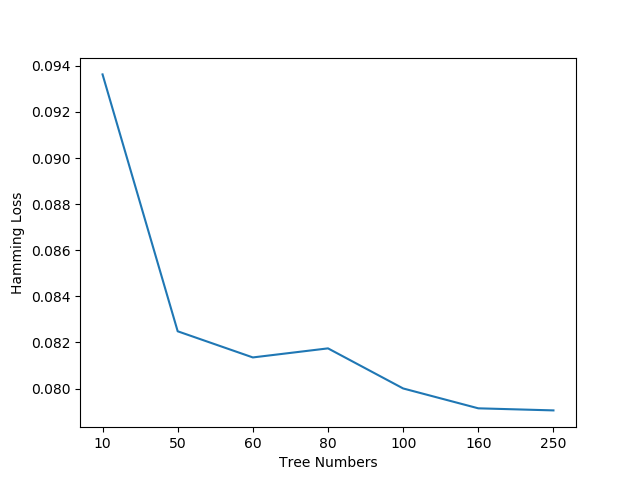
\includegraphics[width=1\linewidth]{label}
\captionof{figure}{Label Powerset performance with different number of trees in base classifier.\\}

It can be easily seen on Table 3 that adding more trees help to get better results. Accuracy increases and loss decreases. We should note that we couldn't add more than 250 trees because of our computer's limited memory. But looking to increase in accuracy or decrease in loss we can say that 250 trees is close to global maxima. We assume that adding more trees to the forest will cause model to overfit the training data. So we stopped at this point.

The most we care about is hamming loss in these metrics since it is more forgiving in terms of evaluation, it doesn't expect the model to predict in the exactly same way with the result. It seems a more correct metric for multi-label classification. So, the current hamming loss results are actually pretty nice, but we aren't satisfied with that. The results with different number of trees is shown in Figure 3.

\subsection{Analysis of ANN}

We have played with the hyper-parameters of the ANN model a lot. But, we will not go through all of that but, will share some of the results. The hyper-parameters we played with are limited with neuron number, batch and epoch number.

\begin{table}[H]
\begin{center}
\begin{tabular}{|c|c|c|c|c|c|}
\hline
Batch size & 2 & 4 & 16 & 32 & 64\\
\hline
10 Epochs & 0.070 & 0.069 & 0.071 & 0.072 & 0.08\\
25 Epochs & 0.070 & 0.071 & 0.072 & 0.072 & 0.075\\
100 Epochs & 0.069 & 0.069 & 0.072 & 0.072 & 0.073\\
1000 Epochs & - & - & - & 0.038 & 0.036\\
\hline
\end{tabular}
\end{center}
\caption{Performance of ANN with different batch sizes and epoch numbers}
\end{table}

The effects of training with different batch size and epochs are shown in Table 4. We got our best results when we trained our model with 1000 epochs. 10, 25 and 100 epochs are simply not enough to train a model properly. They just underfit the training data. As batch size increased accuracy of our models decreased.

\begin{table}[H]
\begin{center}
\begin{tabular}{|c|c|c|c|}
\hline
Neuron Number & 128 & 256 & 512\\
\hline
Threshold-Based Accuracy & 39.8\% & 43.5\% & 37.5\%\\
\hline
\end{tabular}
\end{center}
\caption{Hamming Loss values of our main model with different neuron numbers}
\end{table}

In table 5, the results of ANN's performance with different neuron numbers are shown. As it can be clearly seen 128 neurons underfit and 512 neurons overfit the training data. Thus, we worked with 256 neuron per layer, which seemed to give a good result. A similar result was achieved in Hakan and Sefa's paper\cite{oldpaper} in Section 4, so we did not played with neuron numbers and layer numbers that much.

\subsection{Comparison of Models}

The comparison between our side model(Label Powerset - Random Forest with 250 trees as base classifier) and our main model(ANN - 2 Hidden labels of 256 neurons trained with 1000 epoch and 64 batch size) has done in this section. The results are shown in Table 6.

\begin{table}[H]
\begin{center}
\begin{tabular}{|c|c|}
\hline
Label Powerset & ANN\\
\hline
0.08 & 0.036 \\
\hline
\end{tabular}
\end{center}
\caption{Hamming Loss values of our main model and side model}
\end{table}

Our main model, ANN, performs much better than our side model in our problem. ANN also gives us faster train and test times than Label Powerset. So it can be considered better in any angle.

\subsection{Analysis of Threshold-Based Accuracy}

In this experiment, we have analysed the effect of threshold on the accuracy with one of our models(ANN- 256 Neuron - 2 Layers - 100 Epoch - 64 Batch). We have also made a comparison with hamming loss to explain our metric better.

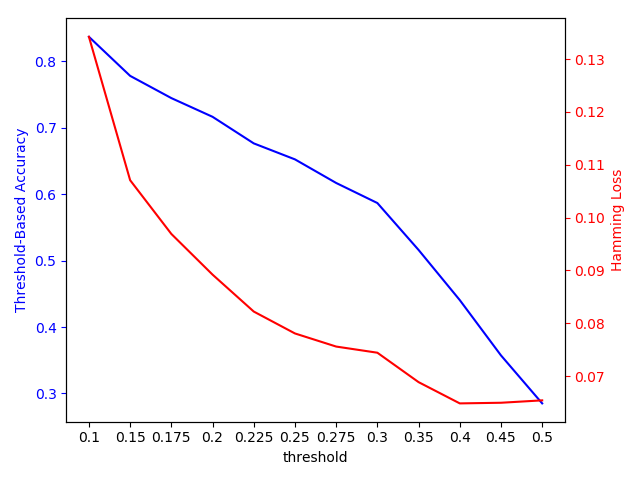
\includegraphics[width=1\linewidth]{hl-th}
\captionof{figure}{Threshold-Based Accuracy and Hamming Loss\\}

The results of the experiment are shown in Figure 4. As you can see as threshold increases our accuracy decrease, but the surprising thing is that hamming loss value also decreases. The explanation is that if the threshold is low more genres will pass the threshold and looking to the graph above we can see that a lot of wrong genres pass the threshold. So as the threshold increases those genres stop passing the threshold so the loss decreases. 

The reason accuracy decreases as well is that the high hit-rate. As the threshold increase the number of genres that can pass it decrease. So it becomes harder for the model to hit enough genres so the percentage can pass the hit-rate. Hit-rate is 0.65, it is a high value, because we have at most 8 genres representing a book. 

\section{Conclusions}
\begin{figure*}
\begin{minipage}{1\linewidth}

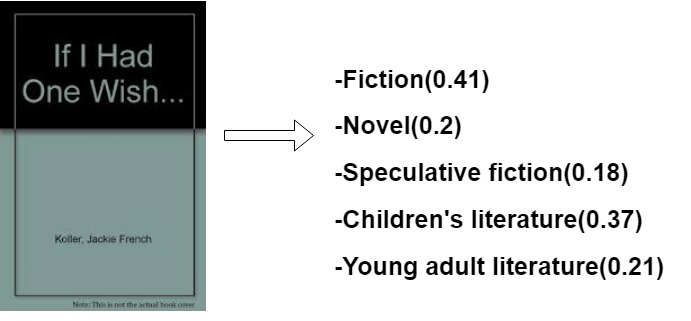
\includegraphics[width=0.3\linewidth]{book1}
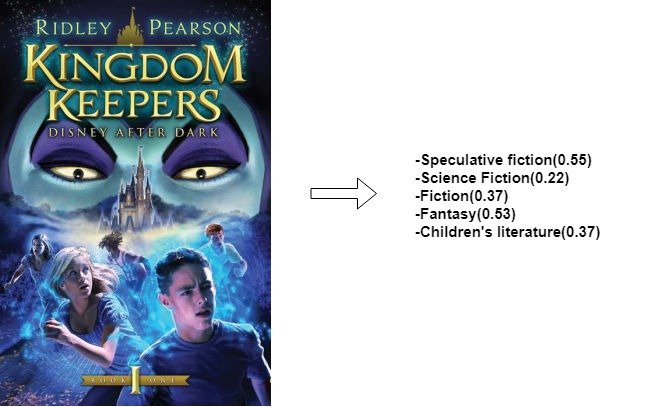
\includegraphics[width=0.4\linewidth]{book2}
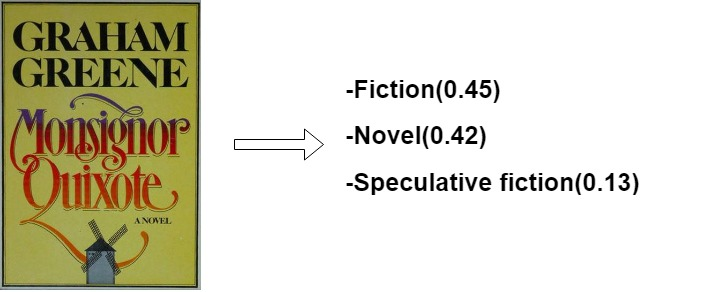
\includegraphics[width=0.3\linewidth]{book3}

\caption{Sample outputs.}

\end{minipage}
\label{fig:short}
\end{figure*}

We have described several approaches to solve and evaluate multi-label classification problems in this paper along with their respective results. While these methods perform rather well, multi-label text classification should not be taken for granted. 

The work done in Hakan and Sefa's previous paper\cite{oldpaper} should be considered as incorrect, because it doesn't fully solve the problem. Considering a book to have only one genre at a time is wrong since it may have multiple genres. Instead, our work discussed in this paper is a much better 
solution that fully grasps the problem.

Improvements over previous ANN model can be tracked to 2 major sources: First, changing output layer's activation function to sigmoid to represent the output vector in bernoulli distribution surprisingly well. Future work should investigate whether better results can be obtained if other distributions are used. Second, changing loss function to binary crossentropy to look each node in output layer independently.

Comparisons on the representation of input show us clearly that Word2Vec model performs much better than Bag of Words model, as expected. Future work should investigate if Doc2Vec will perform even better than Word2Vec, since with Doc2Vec compositional semantics can be got more clearly.

Improvements can be done in Threshold-Based Accuracy. A dynamic 'hit-rate' value can be implemented for much larger scale problems with many more labels to classify. The issue of many of the labels passing threshold should be investigated as well. For example, the model can predict 13 genres that pass threshold to a book with only 6 genres and the correctly predicted genres can pass the hit-rate. In this case, algorithm needs to somehow penalize this prediction. The reasons of this is discussed before in Section 4.6. However, we should note that this can be avoided by giving a really high hit-rate, which is actually a bandage solution which will not get along with the increase of threshold. In our problem, a hit-rate of 0.65 is pretty high looking to the output vectors our ANN model give. But in another problem a hit-rate of 0.9 may need to be given. This way the algorithm would work more dynamically unlike the state it is in right now, which is much more static to our problem and model.

In Figure 5 you can see some of our example outputs. The genres and their probabilities are given in the right side of the images.

{\small
\bibliographystyle{ieee}
\bibliography{Final_Report}
}


\end{document}
